\chapter{Modello a memoria comune}

Esistono due modelli principale di interazione tra i processi:
\begin{itemize}
    \item memoria comune, ambiente globale con memoria condivisa
    \item scambio di messaggi, ambiente locale con memoria distribuita
\end{itemize}

In questo capitolo si analizza il modello a memoria comune.

Il sistema è visto come un insieme di \textbf{processi} e \textbf{oggetti}.

\begin{figure}[H]
    \centering
    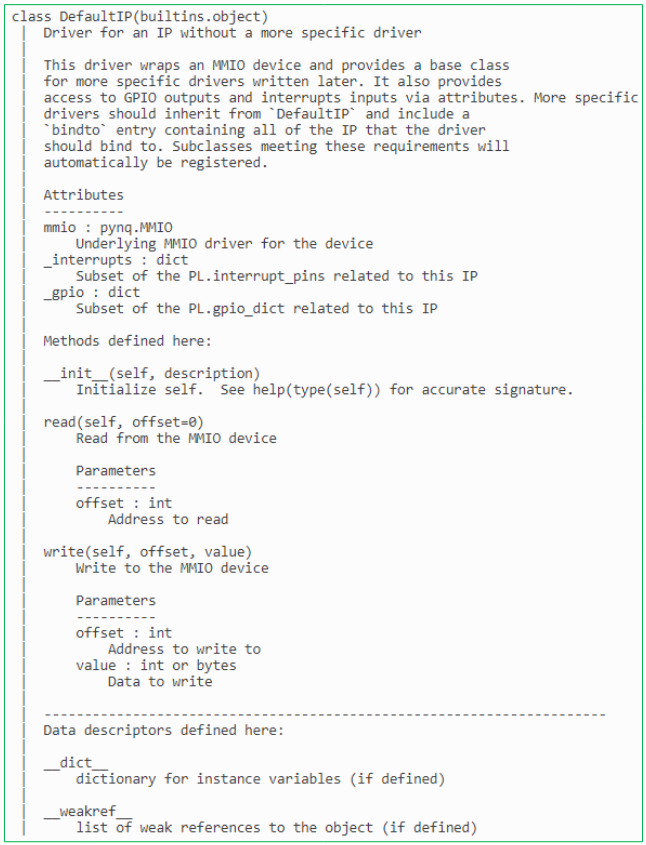
\includegraphics[width=0.5\textwidth]{/home/riccardoob/appunti/sistemi_operativi/images/18.png}
\end{figure}

In questo grafo, O1 e O4 sono risorse private, mentre O2 e O3 sono comuni.

Esistono due tipi di interazione tra processi:
\begin{itemize}
    \item \textbf{competizione}
    \item \textbf{cooperazione}
\end{itemize}

In questo modello, ogni applicazione viene strutturata come uninsieme di componenti, suddiviso in due sottoinsiemi disgiunti, i processi come componenti attivi e le risorse come componenti passivi.

\paragraph{Risorsa} Qualunque oggetto fisico di cui un processo necessita per portare a termine il suo compito.

Le risorse sono raggruppate in \underline{classi}, categorie che identificano l'insieme delle operazioni che un processo può eseguire.

\section{Gestore di una risorsa}

Per ogni risorsa R, il suo \textbf{gestore} definisce, in ogni istante $t$, l'insieme $SR(t)$ dei processi che hanno il diritto di operare su R.

Classificazione delle risorse in base alla condivisione:
\begin{itemize}
    \item \textbf{dedicata} se $SR(t)$ ha una cardinalità sempre $\le 1$
    \item \textbf{condivisa} in caso contrario
\end{itemize}

Classificazione delle risorse in base al tipo di allocazione:
\begin{itemize}
    \item \textbf{allocata staticamente} se $SR(t)$ è una costante $SR(t) = SR(t_0), \forall t$ 
    \item \textbf{allocata dinamicamente} se $SR(t)$ è una funzione del tempo
\end{itemize}
\begin{figure}[H]
    \caption{Tipologia di allocazione delle risorse}
    \centering
    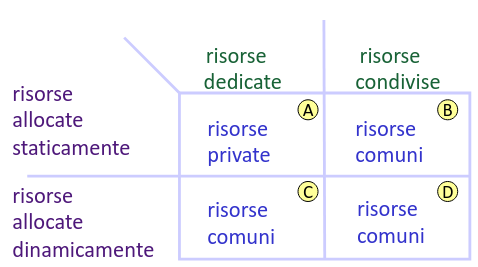
\includegraphics[width=0.65\textwidth]{/home/riccardoob/appunti/sistemi_operativi/images/19.png}
\end{figure}

Per ogni risorsa allocata \textit{staticamente}, l'insieme $SR(t)$ è definito prima che il programma inizi la propria esecuzione, il gestore della risorsa è il programmatore che stabilisce quale processo può operare su R.

Per ogni risorsa allocata \textit{dinamicamente}, il gestore $G_R$ definisce l'insieme $SR(t)$ in fase di esecuzione e quindi deve essere un componenete della stessa applicazione, nel quale l'allocazione viene decisa a run-time in base alle politiche date.

\subsection{Compiti del gestore di una risorsa}
Il gestore di una risorsa deve essere in grado di:
\begin{itemize}
    \item mantenere \textbf{aggiornato} l'insieme $SR(t)$ e lo stato di allocazione della risorsa
    \item fornire i \textbf{meccanismi} che un processo può utilizzare per ottenere i permessi per accedere alla risorsa e quindi entrare a far parte dell'insieme $SR(t)$ e per rilasciare questi permessi
    \item implementare la \textbf{strategia} di allocazione della risorsa e cioè definire quando, a chi e per quanto tempo allocare la risorsa
\end{itemize}

\subsection{Accesso a risorse}
Considerando un processo P che deve operare su una risorsa R di tipo T.

\subsubsection{Allocata staticamente}
Se R è allocata staticamente a P il processo, se appartiene a $SR(t)$ possiede il diritto di operae su R in qualunque istante.

\subsubsection{Allocata dinamicamente}
Se R è allocata dinamicamente a P, è necessario prevedere un gestore GR che implementa le funzioni di \underline{richiesta} e \underline{rilascio}, il processo deve richiedere accesso, eseguire operazione e rilasciare accesso.

\subsubsection{Allocata condivisa}
Se R è allocata come \textit{risorsa condivisa} è necessario assicurare che gli accessi avvengano in modo non divisibile: le funzioni di acecsso alla risorsa devono essere programmate come una classe di sezioni critiche utilizzando meccanismi di sincronizzazione).

\subsubsection{Allocata dedicata}
Se R è allocata come \textit{risorsa dedicata} essendo P l'unico processo che accede alla risorsa, non è necessario prevedere sincronizzazione.

\subsection{Specifica della sincronizzazione}

\paragraph{Regione critica condizionale [Hoare, Brinch-hansen]} Formalismo che consente di esprimere la specifica di qualunque \textbf{vincolo di sincronizzazione}.

\begin{minted}[bgcolor=lightgray,framesep=2mm,baselinestretch=1.2,fontsize=\footnotesize]{c}
region R << Sa; when(C) Sb;>>
\end{minted}

Il corpo della region rappresenta una operazione da eseguire sulla risorsa condivisa R, è la \textbf{sezione critica} che deve essere eseguita in mutua esclusione con le altre operazioni.

Vengono eseguite le istruzioni \texttt{Sa} e, non appena C è vera, \texttt{Sb}.

\begin{figure}[H]
    \centering
    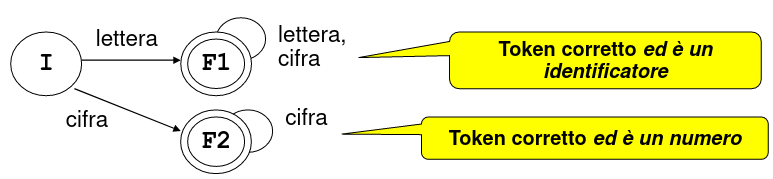
\includegraphics[width=0.5\textwidth]{/home/riccardoob/appunti/sistemi_operativi/images/20.png}
\end{figure}

\subsection{Casi particolari}
\begin{itemize}
    \item \texttt{region R << S; >>} mutua esclusione senza ulteriori vincoli
    \item \texttt{region R << when(C) >>} specifica di un vincolo di sincronizzazione: P deve attendere che C si verifichi
    \item \texttt{region R << when(C) S; >>} in questo caso C è una precondizione necessaria per eseguire S
\end{itemize}

\section{Il problema della mutua esclusione}
Il problema della mutua esclusione nasce quando più processi possono avere accesso a variabili comuni, la regola impone che le operazioni non si sovrappongano nel tempo, nessun vincolo è imposto sull'ordine delle operazioni.

\paragraph{Sezione critica}
Una sequenza di istruzioni che accede e modifica un insieme di variabili comuni prende il nome di sezione critica.

La regola di mutua esclusione stabilisce che sezioni critiche della stessa classe non pososno essere in esecuzione contemporaneamente.

Il protocollo di esecuzione di una sezione critica è il seguente:
\begin{minted}[bgcolor=lightgray,framesep=2mm,baselinestretch=1.2,fontsize=\footnotesize]{c}
<prologo>
S;
<epilogo>
\end{minted}

Nel prologo si richiede e ottiene l'autorizzazione a eseguire la sezione, nell'epilogo si rilascia la risorsa.

\section{Strumenti linguistici per la programmazione di interazioni}

\subsection{Semaforo}
É uno strumento di basso livello, realizzato dal kernel della macchina, utile a risolvere qualsiasi problema di sincronizzazione.

L'eventuale attesa nell'esecuzione può essere realizzata utilizzando i meccanismi di gestione dei thread (sospensione, riattivazione) offerti dal kernel.

Un semaforo è una variabile \textit{interna non negativa} alla quale è possibile accedere solo tramite le due operazioni \texttt{P} e \texttt{V}.

Specifica delle operazioni di un semaforo:
\begin{minted}[bgcolor=lightgray,framesep=2mm,baselinestretch=1.2,fontsize=\footnotesize]{c}
void P(semaphore s):
    region s << when(val>0) val--; >>


void V(semaphore s):
    region s << val++; >>
\end{minted}

Dato un semaforo S, siano:
\begin{itemize}
    \item $\texttt{val}_\texttt{s}$: valore dell'intero non negativo associato al semaforo
    \item $\texttt{I}_\texttt{s}$: valore interno maggiore di zero di inizializzazione
    \item $\texttt{nv}_\texttt{s}$: numero di volte che l'operazione \texttt{V(s)} è stata eseguita
    \item $\texttt{np}_\texttt{s}$: numero di volte che l'operazione \texttt{P(s)} è stata eseguita
\end{itemize}

\subsubsection{Relazione di invarianza}
Ad ogni istante possiamo esprimere il valore del semaforo come $\texttt{val}_\texttt{s} = \texttt{I}_\texttt{s} + \texttt{nv}_\texttt{s} - \texttt{np}_\texttt{s}$ da cui si ottiene $\texttt{np}_\texttt{s}\le \texttt{I}_\texttt{s}+\texttt{nv}_\texttt{s}$

La relazione di invarianza è sempre soddisfatta (safety property), si può usare questa proprietà per dimostrare formalmente le proprietà dei programmi concorrenti.

\subsubsection{Utilizzo}
Il semaforo è uno strumento generale che consente la risoluzione di qualunque problema di sincronizzazione, ne esistono però specializzazioni utili in particolari casi:
\begin{itemize}
    \item semafori mutua esclusione
    \item semafori evento
    \item semafori binari composti
    \item semafori condizione
    \item semafori risorsa
    \item semafori privati
\end{itemize}

\subsubsection{Semaforo mutua esclusione}

Viene inizializzato a 1 ed è usato per realizzare le sezioni critiche di una stessa classe.
\begin{minted}[bgcolor=lightgray,framesep=2mm,baselinestretch=1.2,fontsize=\footnotesize]{java}
class risorsa {
    semaphore mutex = 1;
    public void op1() {
        P(mutex);
        //<sez. critica>
        V(mutex);
    }
}
\end{minted}

Le seguenti condizioni sono soddisfatte:
\begin{itemize}
    \item sezione critiche della stessa classe devono essere eseguite in modo mutualmente esclusivo
    \item non deve essere possibile il verificarsi di deadlock
    \item un processo fuori dalla sezione critica non deve bloccare l'entrata ad altri processi
\end{itemize}

\subsection{Mutua esclusione tra gruppi e processi}
In alcuni casi può essere utile consentire a più processi di eseguire contemporaneamente la stessa operazione su una risorsa, ma non operazioni diverse.

Data la risorsa condivisa \texttt{ris} e indicate con $\texttt{op}_\texttt{1} \dots \texttt{op}_\texttt{n}$ le n operazioni eseguibili su \texttt{ris}, si vuole garantire che i processi possano eseguire contemporaneamente $\texttt{op}_\texttt{i}$.

Lo schema è il solito prologo, operazione, epilogo:
\begin{itemize}
    \item il \underline{prologo} deve sospendere il processo che ha chiamato l'operazione se sulla risorsa sono in esecuzione operazioni diverse, altrimenti deve procedere
    \item l'\underline{epilogo} deve liberare la mutua esclusione solo se il processo che lo esegue è l'unico processo in esecuzione sulla risorsa
\end{itemize}

Si definisce una \textit{semaforo mutex} per la mutua esclusione tra operazioni e un'altro per le sezioni critiche prologo e epilogo.

\begin{minted}[bgcolor=lightgray,framesep=2mm,baselinestretch=1.2,fontsize=\footnotesize]{java}
semaphore mutex=1, m_i=1;

public void op_i() {
    P(m_i);
    cont_i++;
    if (cont_i==1) P(mutex);
    V(m_i);
    //<corpo operazione>
    P(m_i);
    cont_i--;
    if (cont_i==0) V(mutex);
    V(m_i);
}
\end{minted}

Questo schema è applicabile alla casistica di lettura scrittura su file: più processi possono leggere un file contemporaneamente mentre una sola può modificare.

\subsection{Semafori evento - scambio di messaggi temporali}
Un semaforo \textbf{evento} è un semaforo binario utilizzato per imporre un vincolo di precedenza tra operazioni e processi.

\subsubsection{Esempio}
$\texttt{op}_a$ deve essere eseguita da $\texttt{P}_1$ solo dopo che $\texttt{P}_2$ ha eseguito $\texttt{op}_b$.

Si introduce un semaforo \texttt{sem} inizializzato a zero:
\begin{itemize}
    \item prima di eseguire $\texttt{op}_a$, $\texttt{P}_1$ esegue \texttt{P(sem)}
    \item dopo aver eseguite $\texttt{op}_b$, $\texttt{P}_2$ esegue \texttt{V(sem)}
\end{itemize}

\begin{figure}[H]
    \centering
    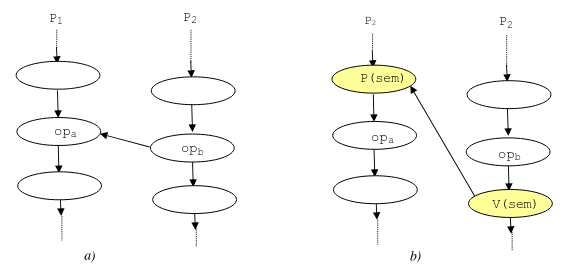
\includegraphics[width=0.6\textwidth]{/home/riccardoob/appunti/sistemi_operativi/images/21.png}
\end{figure}

\subsubsection{Problema del rendez-vous}
Due processi \texttt{P}$_1$ e \texttt{P}$_2$ eseguono ciascuno due operazioni, \texttt{p}$_a$ e \texttt{p}$_b$ il primo e \texttt{q}$_a$ e \texttt{q}$_b$ il secondo.

\begin{mdframed}[topline=false,bottomline=false,rightline=false]
    \textbf{Vincolo di rendez-vous}\\
    L'esecuzione di \texttt{p}$_b$ da parte di \texttt{P}$_1$ e \texttt{q}$_b$ da parte di \texttt{P}$_2$ possno inziare solo dopo che entrambi i processi hanno completato la loro prima operazione( \texttt{p}$_a$ e \texttt{q}$_a$).
\end{mdframed}

Ogni processo segnala quando arriva al punto di incontro e attende, si utilizzano due semafori \texttt{sem1} e \texttt{sem2}.

\begin{figure}[H]
    \centering
    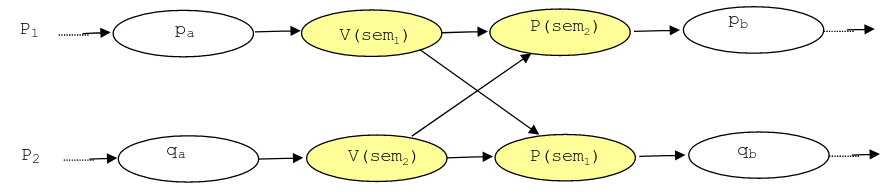
\includegraphics[width=0.6\textwidth]{/home/riccardoob/appunti/sistemi_operativi/images/22.png}
\end{figure}

Si può generalizzare il concetto del rendez-vous a \texttt{N} processi, introducendo il concetto di barriera di sincronizzazione.

\subsubsection{Barriera di sincronizzazione}
L'esecuzione di ogni operazione \texttt{P}$_{ib}$ è subordinata al completamento di tutte le istruzioni \texttt{P}$_{ia} (i=1,\dots,N)$

\begin{figure}[H]
    \centering
    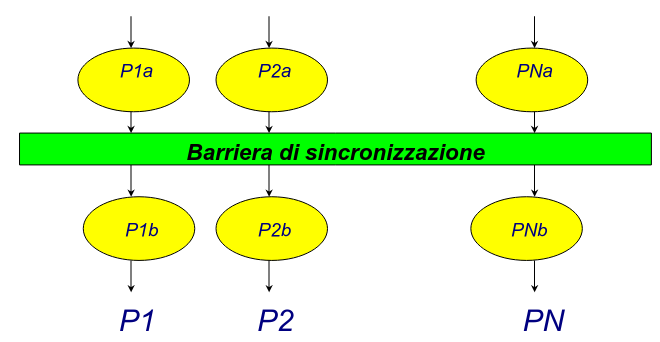
\includegraphics[width=0.6\textwidth]{/home/riccardoob/appunti/sistemi_operativi/images/23.png}
\end{figure}

\begin{minted}[bgcolor=lightgray,framesep=2mm,baselinestretch=1.2,fontsize=\footnotesize]{java}
// condivise
semaphore mutex = 1;
semaphore barriera = 0;
int completati = 0;
//struttura thread i-esimo P_i
p(mutex);
completati++;
if (completati==N)
    v(barriera);
v(mutex);
p(barriera);
v(barriera);
\end{minted}

\subsection{Semafori binari composti - scambio di dati}
Due processi \texttt{P}$_1$ e \texttt{P}$_2$ si scambiano dati di tipo \texttt{T} utilizzando una memoria condivisa.

Gli accessi al buffer devono essere mutuamente esclusivi, \texttt{P}$_2$ può \textit{prelevare} un dato solo dopo che \texttt{P}$_1$ lo ha \textit{inserito}, \texttt{P}$_1$, \textit{prima} di inserire un dato, deve attendere che \texttt{P}$_2$ abbia \textit{estratto} il precedente.

\begin{figure}[H]
    \centering
    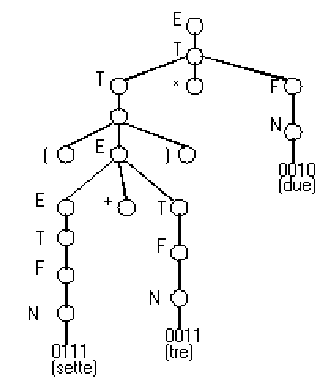
\includegraphics[width=0.6\textwidth]{/home/riccardoob/appunti/sistemi_operativi/images/24.png}
\end{figure}

Per implementare questa funzionalità si utilizzano due semafori:
\begin{itemize}
    \item \texttt{vu}, per realizzare l'attesa di \texttt{P}$_1$ in caso di buffer pieno
    \item \texttt{pn}, per realizzare l'attesa di \texttt{P}$_2$ in caso di buffer vuoto
\end{itemize}

\begin{multicols}{2}
    \begin{minted}[bgcolor=lightgray,framesep=2mm,baselinestretch=1.2,fontsize=\footnotesize]{java}
void invio(T dato) {
    P(vu);
    inserisci(dato);
    V(pn);
}


//P1
while (true) {
    //prepara messaggio
    invio(msg);
}
    \end{minted}
    \columnbreak
    \begin{minted}[bgcolor=lightgray,framesep=2mm,baselinestretch=1.2,fontsize=\footnotesize]{java}
T ricezione() {
    T dato;
    P(pn);
    dato = estrai();
    V(vu);
    return dato;
}
//P2
while (true) {
    M = ricezione();
    //consuma
}
    \end{minted}
\end{multicols}

\begin{mdframed}[topline=false,bottomline=false,rightline=false]
    Un semaforo binario composto è un insieme di semafori usato in modo tale che:
    \begin{itemize}
        \item uno solo di essi sia inizializzato a 1 e tutti gli altri a 0
        \item ogni processo che usa questi semafori esegue sempre sequenze che iniziano con la P su uno di questi e termina con la V su un altro
    \end{itemize}
\end{mdframed}
\subsection{Semafori condizione}
In alcuni casi, l'esecuzione di una istruzione \texttt{S}$_1$ su una risorsa \texttt{R} è subordinata a una condizione \texttt{C} 
\begin{minted}[bgcolor=lightgray,framesep=2mm,baselinestretch=1.2,fontsize=\footnotesize]{C}
void op1(): region R << when(C) S1; >>
\end{minted}
\begin{itemize}
    \item \texttt{op1()} è una regione critica
    \item \texttt{S1} ha come precondizione la validità della condizione logica \texttt{C}
\end{itemize}

Il processo deve sospendersi se la condizione non si verifica, e deve uscire dalla regione per permettere ad altri processi di eseguire operazioni su \texttt{R} per rendere vera la condizione \texttt{C}.

\begin{figure}[H]
    \centering
    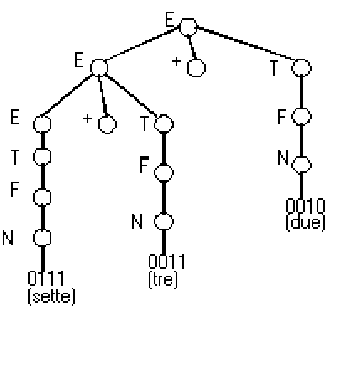
\includegraphics[width=0.7\textwidth]{/home/riccardoob/appunti/sistemi_operativi/images/25.png}
\end{figure}

Lo schema \texttt{(a)} presuppone una forma di attesa attiva da parte del processo che non trova soddisfatta la condizione.

Nello schema \texttt{(b)} si realizza la region \textbf{sospendendo} il processo sul semaforo \texttt{sem} da associare alla condizione, si rende necessaria un'altra operazione \texttt{op2} che abbia \texttt{C} come postcondizione e che chiami nel suo contesto \texttt{V(sem)}.

\vspace{-0.5cm}
\subsubsection{Schema attesa circolare}
\vspace{-0.5cm}
\begin{multicols}{2}
    \begin{minted}[bgcolor=lightgray,framesep=2mm,baselinestretch=1.2,fontsize=\footnotesize]{java}
public void op1() {
    P(mutex);
    while (!C) {
        csem++;
        V(mutex);
        P(sem);
        P(mutex);
    }
    S1;
    V(mutex);
}
    \end{minted}
    \columnbreak
    \begin{minted}[bgcolor=lightgray,framesep=2mm,baselinestretch=1.2,fontsize=\footnotesize]{c}
public void op2() {
    P(mutex);
    if (csem > 0) {
        csem--;
        V(sem);
    }
    V(mutex);
}
    \end{minted}
\end{multicols}

\subsubsection{Schema passaggio testimone}

\begin{multicols}{2}
    \begin{minted}[bgcolor=lightgray,framesep=2mm,baselinestretch=1.2,fontsize=\footnotesize]{java}
public void op1() {
    P(mutex);
    if (!C) {
        csem++;
        V(mutex);
        P(sem);
        csem--;
    }
    S1;
    V(mutex);
}
    \end{minted}
    \columnbreak
    \begin{minted}[bgcolor=lightgray,framesep=2mm,baselinestretch=1.2,fontsize=\footnotesize]{java}
public void op2() {
    P(mutex);
    S2;
    if (C && csem > 0)
        V(sem);
    else
        V(mutex);
}
    \end{minted}
\end{multicols}

Il metodo del testimone è il più efficiente, tuttavia è possibile risvegliare \textit{un solo} processo alla volta e la condizione \texttt{C} non può dipendere da parametri locali a \texttt{op1()}.

\subsubsection{Gestione di un pool di risorse equivalenti}

Si consideri un \textbf{pool} di \texttt{N} risorse tutte uguali, ciascun processo può operare su una qualsiasi risorsa del pool, purché \textit{libera}.

É necessario un \textbf{gestore} che mantenga aggiornato lo stato delle risorse:
\begin{itemize}
    \item ogni processo, prima di operare su una risorsa \textit{chiede al gestore} l'allocazione di una di esse
    \item il gestore \textbf{assegna} al processo una risorsa libera, passandogli l'\textbf{indice} relativo
    \item il processo opera sulla risorsa
    \item al termine il processo \textbf{rilascia} la risorsa a gestore
\end{itemize}

\begin{minted}[bgcolor=lightgray,framesep=2mm,baselinestretch=1.2,fontsize=\footnotesize]{java}
class Gestore {
    semaphore mutex = 1;
    semaphore sem = 0;
    int csem = 0;
    boolean libera[N];
    int disponibili = N;
    {for (int i = 0; i < N; i++) libera[i]=true;}
    
    public int richiesta() {
        int i = 0;
        P(mutex);
        if (disponibili == 0) {
            csem++;
            V(mutex);
            P(sem);
            csem--;
        }
        while (!libero[i]) i++;
        libero[i] = false;
        V(mutex);
        return i;
    }

    public void rilascio(int r) {
        P(mutex);
        libero[r] = true;
        disponibili++;
        if (csem > 0) 
            V(sem);
        else 
            V(mutex);
    }
}
\end{minted}

Schema di esempio di un generico processo che vuole accedere a una risorsa \texttt{ris}.

\begin{minted}[bgcolor=lightgray,framesep=2mm,baselinestretch=1.2,fontsize=\footnotesize]{java}
process P {
    int ris;
    ...
    ris = G.richiesta();
    //<utilizzo risorsa>
    G.rilascio();
    ...
}
\end{minted}

\subsection{Semaforo risorsa}
I semafori risorsa sono semafori generali, ovvero possono assumere qualunque valore maggiore di zero.

Sono utilizzato per realizzare allocazione per risorse equivalenti, il valore del semaforo rappresenta il \textbf{numero di risorse libere}.

\subsubsection{Gestione di un pool di risorse equivalenti}
Si può utilizzare un semaforo risorsa per gestire un pool di risorse, si crea un unico semaforo \texttt{n\_ris} inizializzato con un valore uguale al numero di risorse, si eseguono P(n\_ris) in allocazione e V(n\_ris) in rilascio.

\begin{minted}[bgcolor=lightgray,framesep=2mm,baselinestretch=1.2,fontsize=\footnotesize]{java}
class Gestore {
    semaphore mutex = 1;
    semaphore n_ris = N;
    boolean libero[N];

    {for (int i = 0; i < N; i++)
        libera[i] = true;}

    public int richiesta() {
        int i = 0;
        P(n_ris);
        P(mutex);
        while (!libero[i]) i++;
        libero[i] = false;
        V(mutex);
        return i;
    }
    
    public void rilascio (int r) {
        P(mutex);
        libero[r] = true;
        V(mutex);
        V(n_ris);
    }

}
\end{minted}

\subsubsection{Problema dei produttori/consumatori}
Si crea un buffer di \texttt{n} elementi, strutturato come una coda
\begin{minted}[bgcolor=lightgray,framesep=2mm,baselinestretch=1.2,fontsize=\footnotesize]{java}
coda_di_n_T buffer;
semaphore pn = 0;
semaphore vu = 0;
semaphore mutex = 1;
\end{minted}

\begin{multicols}{2}
    \begin{minted}[bgcolor=lightgray,framesep=2mm,baselinestretch=1.2,fontsize=\footnotesize]{java}
void invio(T dato) {
    P(vu);
    P(mutex);
    buffer.inserisci(dato);
    V(mutex);
    V(pn);
}
    \end{minted}
    \columnbreak
    \begin{minted}[bgcolor=lightgray,framesep=2mm,baselinestretch=1.2,fontsize=\footnotesize]{java}
void ricezione() {
    T dato;
    P(pn);
    P(mutex);
    dato = buffer.estrai();
    V(mutex);
    V(vu);
    return dato;
}
    \end{minted}
\end{multicols}

\subsection{Semafori privati - specifiche strategie di allocazione}
Qualora si voglia realizzare una politica di gestione delle risorse particolare, la decisione se permettere o no l'esecuzione a un dato processo dipende dal verificarsi duna specifica \textbf{condizione di sincronizzazione}.

Queste condizioni vengono espresse in termini di variabili che rappresentano lo \textbf{stato della risorsa} e variabili \textit{locali} ai singoli processi.

Sorge il problema di quale processo mettere in esecuzione, risolvibile definendo una \textbf{politica di risveglio} dei processi bloccati.

Nei casi precedenti la politica di risveglio era dipendente dalla specifica implementazione dell'algoritmo all'interno della V, solitamente realizzato con risveglio FIFO.

\begin{mdframed}[topline=false,bottomline=false,rightline=false]
    Un semaforo \texttt{s} si dice \textbf{privato} per un processo quando solo tale processo può eseguire la primitiva \texttt{P} su semaforo \texttt{s}. La primitiva \texttt{V} può essere eseguita da qualunque processo.
\end{mdframed}

Un semaforo privato viene inizializzato con valore \textbf{zero}.

Il processo che acquisisce la risorsa può sospendersi sul suo semaforo privato se la condizione di sincronizzazione non è soddisfatta, chi rilascia tale risorsa, può risvegliare uno dei processi sospesi (in base alla politica definita) mediante una \texttt{V} sul semaforo privato del processo scelto.

Schema generale:

\begin{minted}[bgcolor=lightgray,framesep=2mm,baselinestretch=1.2,fontsize=\footnotesize,escapeinside=||,mathescape=true]{java}
class Gestore {
    //<struttura dati gestore>;
    semaphore mutex = 1;
    semaphore priv[n] = {0, 0, |$\dots$|, 0} //semafori privati

    public void acquisizione (int i) {
        P(mutex);
        if (/*<condizione di sincronizzazione>)*/ {
            //<allocazione della risorsa>;
            V(priv[i]);
        }
        else {
            //<registrare la sospensione del processo>;
        }
        V(mutex);
        P(priv[i]);
    }

    public void rilascio() {
        int i;
        P(mutex);
        //<rilascio risorsa>;
        if (/*<min 1 processo soddisfa sync condition>*/) {
            //<scelta tra sospesi del Pi da riattivare>;
            //<allocazione risorsa a Pi>;
            //<registrare Pi come non sospeso>;
            V(priv[i]);
        }
        V(mutex);
    }
}
\end{minted}

La sospensione del processo in acqusizione, se la condizione di sincronizzazione non è soddisfatta, deve avvenire \textit{al di fuori dell sezione critica}, altrimenti si impedirebbe a un processo che rilascia la risorsa di accedere a sua volta alla sezione critica.

La soluzione mostrata può presentare inconvenienti:
\begin{itemize}
    \item la \texttt{P} sul privato viene \textbf{sempre eseguita}, anche se non necessario
    \item il codice dell'assegnazione della risorsa è \textit{duplicato} nelle due procedure
\end{itemize}

Correggendo questi problemi:

\begin{minted}[bgcolor=lightgray,framesep=2mm,baselinestretch=1.2,fontsize=\footnotesize]{java}
class Gestore() {
    //<struttura dati gestore>;
    semaphore mutex = 1;
    semaphore priv[n] = {0, 0, |$\dots$|, 0}; //semafori privati

    public void acqusizione(int i) {
        P(mutex);
        if (! //<condizione di sincronizzazione) {
            //<registrare sospensione processo>;
            V(mutex);
            P(priv[i]);
            //<registrare processo come non sospeso>;
        }
        //<allocazione risorsa>;
        V(mutex);
    }

    public void rilascio() {
        int i;
        P(mutex);
        //<rilascio risorsa>;
        if (/*<min 1 processo soddisfa sync condition>*/) {
            //<scelta tra sospesi del Pi da riattivare>;
            V(priv[i]);
        }
        else
            V(mutex);
    }
}
\end{minted}

Il risveglio segue lo schema del \textbf{passaggio del testimone}.

A differenza della soluzione precedente è più complesso realizzare la riattivazione di più processi che hanno condizione di sincronizzazione verificata: il processo che rilascia la risorsa attiva al massimo un processo, il quale dovrà a sua volta provvedere a riattivare eventuali processi.

\subsubsection{Esempio 1}
Su un buffer di N celle di memoria, più produttori possono depositare messaggio di dimensione diversa.

\textbf{Politica di gestione}: tra più produttori ha priorità di accesso quello che fornisce il messaggio di dimensione maggiore.

\textbf{Condizione di sincronizzazione}: il deposito può avvenire se c'è abbastanza spazio per memorizzare il messaggio e non ci sono produttori in attesa.

Il \textbf{prelievo} di messaggi da parte di un consumatore riattiva il produttore con messaggio con \textbf{dimensione maggiore} (se spazio sufficiente nel buffer), se lo \textit{spazio non è sufficiente}, nessun produttore viene riattivato.

Soluzione:
\begin{minted}[bgcolor=lightgray,framesep=2mm,baselinestretch=1.2,fontsize=\footnotesize,escapeinside=||,mathescape=true]{java}
class Buffer {
    int richiesta[num_proc] = 0; //numero di celle richieste da Pi
    int sospesi = 0;
    int vuote = n; //numero celle vuote del buffer

    semaphore mutex = 1;
    semaphore priv[num_proc] = {0, 0, |$\dots$|, 0};

    public void acqusizione(int m, int i) {
        // m dim mess, i id processo
        P(mutex);
        if (sospesi == 0 && vuote >= m) {//assegna m celle a Pi
            vuote = vuote - m;
            V(priv[i]);
        }
        else {
            sospesi++;
            richiesta[i] = m;
        }
        V(mutex);
        P(priv[i]);
    }
    
    public void rilascio(int m) {
        int k;
        P(mutex);
        vuote += m;
        while (sospesi != 0) {
            //<individuazione del Pk con max richiesta>;
            if (richiesta[k] <= vuote) { //assegno a Pk
                vuote = vuote - richiesta[k];
                richiesta[k] = 0;
                sospesi--;
                V(priva[k]);
            }
            else {
                break;
            }
        }
        V(mutex);
    }
}
\end{minted}

\subsubsection{Esempio 2}
Un insieme di processi utilizza un insieme di risorse comuni R1, R2, \dots, Rn. Ogni processo può utilizzare una qualunque delle risorse.

\textbf{Politica di gestione}: a ogni processo è assegnata una \textbf{priorità}, in fase di riattivazione dei processi sospesi, viene scelto quello con la \textit{massima priorità}.

\textbf{Condizione sincronizzazione}: accesso consentito solo se esiste una \textit{risorsa libera}.

Soluzione:

Variabili introdotte
\begin{itemize}
    \item \texttt{PS[i]}: vero se il processo \texttt{Pi} è sospeso, falso altrimenti
    \item \texttt{libera[j]}: falso se la risorsa j-esima è occupata, vero altrimenti
    \item \texttt{disponibili}: numero delle risorse non occupate
    \item \texttt{sospesi}: numero di processi sospesi
    \item \texttt{mutex}: semaforo di mutua esclusione
    \item \texttt{priv[i]}:semafori privati del processo \texttt{Pi}
\end{itemize}

\begin{minted}[bgcolor=lightgray,framesep=2mm,baselinestretch=1.2,fontsize=\footnotesize,escapeinside=||,mathescape=true]{java}
class Gestore {
    semaphore mutex = 1;
    semaphore priv[num_proc] = {0, 0, |$\dots$|, 0};
    int sospesi = 0;
    boolean PS[num_proc] = {false, false, |$\dots$|, false};
    int disponibili = num_ris;
    boolean libera[num_ris] = {true, true, |$\dots$|, false};

    public int richiesta(int proc) {
        int i = 0;
        P(mutex);
        if (disponibili == 0) {
            sospesi++;
            PS[proc] = true;
            V(mutex);
            P(priv[proc]);
            PS[proc] = false;
            sospesi--;
        }
        while (! libera[i]) i++;
        libera[i] = false;
        disponibili--;
        V(mutex);
        return i;
    }

    public void rilascio(int r) {
        P(mutex);
        libera[r] = true;
        disponibili++;
        if (sospesi > 0) {
            //<seleziona il processo Pj a massima priorità tra i sospesi>
            V(priv[j]);
        }
        else V(mutex);
    }
}
\end{minted}

\section{Realizzazione dei semafori}

Nei sistemi multiprogrammati, il semaforo è realizzato dal kernel, che usa i meccanismi di gestione dei processi per evitare attesa attiva.

Si può definire le funzioni \texttt{P} e \texttt{V} in questo modo, garantendo le proprietà del semaforo.

\begin{figure}[H]
    \centering
    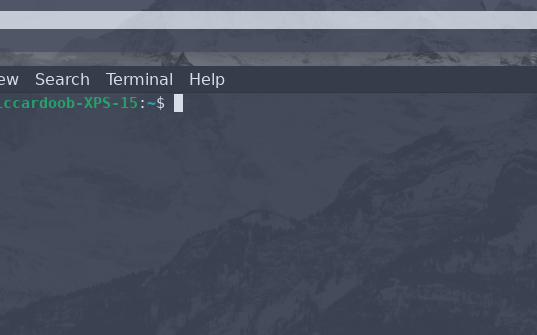
\includegraphics[width=0.8\textwidth]{/home/riccardoob/appunti/sistemi_operativi/images/30.png}
\end{figure}

Un semaforo è identificato dal suo descrittore, definito come segue:
\begin{minted}[bgcolor=lightgray,framesep=2mm,baselinestretch=1.2,fontsize=\footnotesize,escapeinside=||,mathescape=true]{c}
typedef struct {
    int contatore;
    coda queue;
} semaforo;
\end{minted}

Una \texttt{P} su un semaforo con \textit{contatore a 0}, \textit{sospende} il processo nella coda \texttt{queue}, altrimenti il \textit{contatore viene decrementato}.

Una \texttt{V} su un semaforo con \textit{coda non vuota}, \textit{estrae} un processo dalla coda, altrimenti \textit{incrementa il contatore}.

\subsection{Architettura monoprocessore}
Considerando interruzioni disabilitate (per garantire l'atomicità), l'implementazione di \texttt{P} e \texttt{V} sono:

\begin{minted}[bgcolor=lightgray,framesep=2mm,baselinestretch=1.2,fontsize=\footnotesize,escapeinside=||,mathescape=true]{c}
void P(semaphore s) {
    if (s.contatore == 0)
        //<sospensione del processo nella coda associata a s>;
    else
        s.contatore++;
}

void V(semaphore s) {
    if (s.queue != NULL)
        //<estrazione del primo processo dalla coda a s.queue e impostazione a stato di ready>
    else
        s.contatore--;
}
\end{minted}



















































































